\documentclass[10pt,twocolumn]{article}
\usepackage[margin=0.70in]{geometry}
\usepackage[T1]{fontenc}
\usepackage[utf8]{inputenc}
\usepackage{microtype}
\usepackage{amsmath,amssymb,amsthm,mathtools}
\usepackage{booktabs}
\usepackage{graphicx}
\usepackage{subcaption}
\usepackage{xcolor}
\usepackage{hyperref}
\usepackage{enumitem}
\hypersetup{colorlinks=true,linkcolor=blue!50!black,citecolor=blue!50!black,urlcolor=blue!50!black}

\setlength{\columnsep}{0.22in}
\setlength{\textfloatsep}{8pt plus 2pt minus 2pt}
\setlength{\floatsep}{8pt plus 2pt minus 2pt}
\setlength{\intextsep}{8pt plus 2pt minus 2pt}
\setlength{\abovecaptionskip}{4pt}
\setlength{\belowcaptionskip}{0pt}
\setlength{\abovedisplayskip}{5pt}
\setlength{\belowdisplayskip}{5pt}
\captionsetup{font=small}
\raggedbottom

\newtheorem{proposition}{Proposition}
\newtheorem{claim}{Claim}
\newtheorem{remark}{Remark}
\newcommand{\R}{\mathbb{R}}
\newcommand{\E}{\mathbb{E}}
\newcommand{\1}{\mathbf{1}}
\newcommand{\rank}{\operatorname{rank}}
\newcommand{\im}{\operatorname{Im}}
\newcommand{\diag}{\operatorname{Diag}}
\newcommand{\cF}{\mathcal{F}}
\newcommand{\cP}{\mathcal{P}}
\newcommand{\cV}{\mathcal{V}}
\newcommand{\cE}{\mathcal{E}}
\newcommand{\wh}{\widehat}
\newcommand{\dd}{\mathrm{d}}

\title{Low-Rank Path Constraints, CPWL Face Moments, and Fourier Scaling Laws}
\author{Anonymous Workshop Submission}
\date{}

\begin{document}
\maketitle
\vspace{-2.0em}

\begin{abstract}
We revisit the conjecture that low-rank ReLU networks have a better Fourier-space behavior because they create fewer independent path constraints.  The literal graph path count is not the right invariant: factorizing a layer can add latent linear paths.  The right invariant is the dimension of the span of active path coefficients.  We derive a path-space rank constraint, translate it into a normal-subspace constraint for CPWL linear regions, and obtain a face-moment shell law
\[
S_f(\rho)\lesssim \sum_{q=1}^d M_q(f)\rho^{-2(q+1)},
\]
where $M_q$ is a weighted moment of codimension-$q$ faces.  This predicts that low rank should suppress high-codimension intersections and flatten the finite-resolution Fourier slope by leaving the spectrum closer to the facet-dominated $\rho^{-4}$ regime.  We then stress-test the story experimentally.  In random 3D CPWL networks, rank-$2$ bottlenecks reduce an 8-way junction proxy from $0.449$ to $0.062$ and flatten shell slopes from $-6.70$ to $-6.34$.  In 1D, the raw CPWL exponent remains near $-4$, as theory requires; the visible gain instead appears in the learned Fourier transfer function.  A width-$2^{15}$ Fourier/kernel experiment sweeping ranks $1,\ldots,50$ plus a full-rank endpoint shows a clear intermediate optimum: rank $4$ beats the full endpoint on sparse mixtures ($0.250$ vs. $0.461$ MSE, recovery slope $-0.29$ vs. $-0.94$) and dense mixtures ($0.443$ vs. $0.654$ MSE, recovery slope $-0.29$ vs. $-1.20$).  The same optimum is predicted by an approximation-plus-optimization bound.
\end{abstract}

\section{The original conjecture, made precise}
The motivating picture is simple.  A ReLU network is continuous piecewise affine (CPWL).  Its Fourier transform can be decomposed into contributions from faces of the induced polyhedral complex.  Low-dimensional face intersections generate fast-decaying shell terms, while facets generate the slowest CPWL tail.  If low rank reduces the number of independent switching constraints, then the complex should have relatively more high-dimensional faces and fewer deep intersections.  The observed shell spectrum should then decay less steeply at finite resolution.

This paper keeps that geometric story but replaces the informal phrase ``fewer paths'' by a precise one: \emph{fewer independent path coefficients}.  For a layer $W_\ell=U_\ell V_\ell^\top$ with rank $r_\ell$, the computational graph may contain extra latent nodes, yet the active path tensor cannot have mode-rank larger than $r_\ell$.  The rank constraint therefore contracts the space of possible path sums.  That contraction is the bridge from algebra to geometry.

\paragraph{What we validate.}
We focus on three predictions.
\begin{enumerate}[leftmargin=1.2em,itemsep=1pt,topsep=2pt]
\item Low rank should lower high-codimension face moments $M_q$, especially $q\ge2$.
\item In $d\ge2$, this should flatten finite-resolution Fourier shell slopes.
\item In $d=1$, the CPWL tail exponent is pinned near $-4$; the gain should instead appear as a flatter \emph{training transfer function} across Fourier modes and an intermediate optimal rank.
\end{enumerate}
The last point is important: if a 1D experiment does not show a large raw exponent change, that is not a failure of the theory.  It is exactly what a CPWL Fourier expansion predicts.

\begin{figure*}[t]
\centering
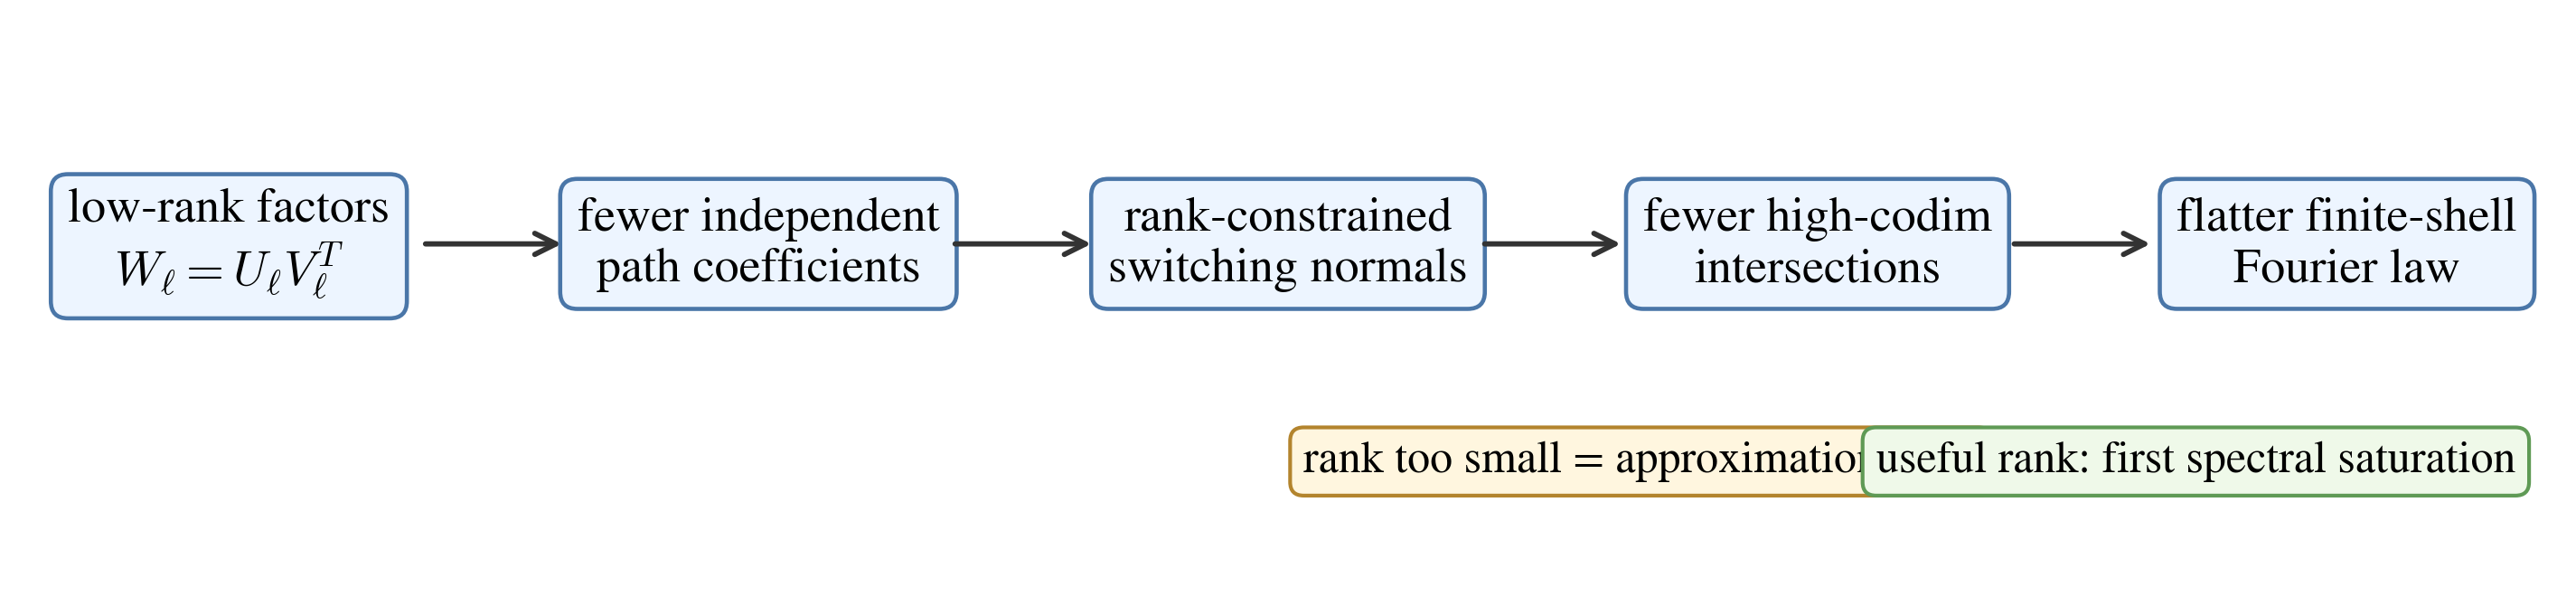
\includegraphics[width=\textwidth]{figures/mechanism.png}
\caption{Central mechanism.  The paper is not claiming fewer graph-theoretic paths.  It claims fewer independent path coefficients, which constrain switching normals, suppress high-codimension CPWL faces, and improve finite-resolution Fourier behavior until approximation error dominates.}
\label{fig:mechanism}
\end{figure*}

\section{Rank constraints in path space}
Consider an $L$-hidden-layer ReLU network
\begin{equation}
 h_\ell(x)=\sigma(W_\ell h_{\ell-1}(x)+b_\ell),\qquad h_0(x)=x\in\R^d,
\end{equation}
with scalar output $f(x)=w_{L+1}^\top h_L(x)+b_{L+1}$ and factorized hidden matrices $W_\ell=U_\ell V_\ell^\top$, $\rank(W_\ell)\le r_\ell$.  On an activation region $R_\varepsilon$,
\begin{equation}
 f(x)=a_\varepsilon^\top x+c_\varepsilon,\qquad
 a_\varepsilon^\top=w_{L+1}^\top D_{L,\varepsilon}W_L\cdots D_{1,\varepsilon}W_1,
\end{equation}
where $D_{\ell,\varepsilon}$ is a diagonal gate matrix.

Expanding $a_\varepsilon$ as a sum over active paths gives coefficients of the form
\begin{equation}
 c_{i_1,\ldots,i_L,j}(\varepsilon)=w_{L+1,i_L}\prod_{\ell=1}^L D_{\ell,i_\ell}(\varepsilon) W_{\ell,i_\ell i_{\ell-1}},
\end{equation}
with $i_0=j$.  If $W_\ell=U_\ell V_\ell^\top$, then along every layer index $i_\ell$ this tensor factors through an $r_\ell$-dimensional latent coordinate.

\paragraph{High-level mechanism.}
The useful interpretation is that a low-rank network has fewer \emph{independent} paths in the sum-over-paths formulation.  The number of symbolic graph paths can remain large, and a factorization may even introduce latent two-hop paths, but their coefficients are no longer free.  If $W_\ell=U_\ell V_\ell^\top$ with rank $r_\ell$, every path coefficient passing through layer $\ell$ factors through an $r_\ell$-dimensional latent coordinate.  Hence low rank means fewer independent path coefficients, not literally fewer drawn edges.

This is the bridge to spectral bias.  Fewer independent path coefficients create fewer independent constraints on the linear-region polytopes of the CPWL network.  Fewer independent constraints suppress low-dimensional, high-codimension intersections and leave relatively more high-dimensional faces.  Since the Fourier contribution of a codimension-$q$ face scales like $\rho^{-2(q+1)}$ in shell energy, suppressing high-codimension moments pushes the observed finite-resolution spectrum toward the lower-decay, facet-dominated $\rho^{-4}$ regime.

\section{From path constraints to CPWL face moments}
The path-space constraint becomes geometric through switching hyperplanes.  Fix a cell of the first $\ell-1$ layers and write
\begin{equation}
 h_{\ell-1}(x)=B_{\ell-1,\varepsilon}x+c_{\ell-1,\varepsilon}.
\end{equation}
For neuron $i$ in layer $\ell$,
\begin{equation}
 a_{\ell i}(x)=u_{\ell i}^\top V_\ell^\top B_{\ell-1,\varepsilon}x+\mathrm{const.}
\end{equation}
Thus the input-space normal is
\begin{equation}
 n_{\ell i\varepsilon}=B_{\ell-1,\varepsilon}^\top V_\ell u_{\ell i}
 \in \cV_{\ell,\varepsilon}:=\im(B_{\ell-1,\varepsilon}^\top V_\ell),
\end{equation}
with
\begin{equation}
 \dim \cV_{\ell,\varepsilon}\le \min(d,r_1,\ldots,r_\ell).
\end{equation}
The possible new cuts inside a cell therefore come from a subspace of normals whose dimension is rank-controlled.

Let $\cF_q(f)$ denote the codimension-$q$ faces of the CPWL complex of $f$.  Define a Fourier-relevant face moment
\begin{equation}\label{eq:Mq}
M_q(f)=\sum_{F\in\cF_q(f)} \|\Delta_F\|^2\,\operatorname{vol}_{d-q}(F)^2\,\omega_F,
\end{equation}
where $\Delta_F$ is the jump of the appropriate directional derivative across the local fan around $F$, and $\omega_F$ is an angular factor.  The exact constants are not the point; the important quantity is how much weighted mass sits on codimension $q$.

\begin{proposition}[subspace arrangement proxy]
Suppose $m$ candidate switches inside a cell have normals contained in a $\rho$-dimensional subspace.  Then a generic arrangement proxy for codimension-$q$ descendants is
\begin{equation}\label{eq:arrangement}
N_q(m,\rho)\le \binom{m}{q}\sum_{j=0}^{\rho-q}\binom{m-q}{j},\qquad q\le \rho,
\end{equation}
and $N_q(m,\rho)=0$ for $q>\rho$.  Hence lowering the effective normal dimension suppresses high-codimension faces first.
\end{proposition}

Combining \eqref{eq:Mq} and \eqref{eq:arrangement} gives the working scaling proxy
\begin{equation}\label{eq:Mqproxy}
M_q(r)\lesssim C_q(r)\binom{m}{q}\sum_{j=0}^{\rho(r)-q}\binom{m-q}{j},
\end{equation}
where $C_q(r)$ captures the size of derivative jumps.  This formula is deliberately conservative: it does not need exact face counts to predict that low-rank bottlenecks hit $q\ge2$ moments before they destroy all facets.

\section{Fourier shell law for CPWL networks}
The proof follows the same path as the spectral-decay theorem of Rahaman et al.~\cite{rahaman2019spectral}, but we keep the face coefficients explicit because these are the quantities affected by rank.  Let $g=\chi f$ be the network restricted to a smooth compact observation window.  On each activation cell $P_\varepsilon$,
\begin{equation}
g(x)=\sum_\varepsilon \chi(x)(a_\varepsilon^\top x+b_\varepsilon)\mathbf 1_{P_\varepsilon}(x).
\end{equation}
The cutoff removes the distributional tail of the global ReLU function, so $\wh g$ is an ordinary Fourier transform.

\begin{proposition}[face Fourier expansion]
\label{prop:face-fourier}
Let $\mathcal F_q(f)$ be the codimension-$q$ faces of the CPWL complex.  For $\xi=\rho\theta$ with $\theta\in\mathbb S^{d-1}$ and $\rho\to\infty$,
\begin{equation}\label{eq:facefourier}
\wh g(\rho\theta)
=
\sum_{q=1}^{d}\rho^{-(q+1)}
\sum_{F\in\mathcal F_q(f)}
A_F(\rho,\theta)
+O(\rho^{-(d+2)}),
\end{equation}
where $A_F$ is an oscillatory integral over $F$ controlled by the derivative jump $\Delta_F$ around the local fan:
\begin{equation}
|A_F(\rho,\theta)|
\le C_\chi\|\Delta_F\|\operatorname{vol}_{d-q}(F)\omega_F(\theta).
\end{equation}
\end{proposition}

\begin{proof}
Write $u_\varepsilon(x)=\chi(x)(a_\varepsilon^\top x+b_\varepsilon)$ on each cell $P_\varepsilon$.  Since $\chi$ is compactly supported,
\begin{equation}
\wh g(\rho\theta)=
\sum_\varepsilon
\int_{P_\varepsilon}e^{-i\rho\langle\theta,x\rangle}
u_\varepsilon(x)\,dx
\end{equation}
is an ordinary oscillatory integral.  With $D_\theta=\theta\cdot\nabla$ and
$D_\theta e^{-i\rho\langle\theta,x\rangle}=-i\rho e^{-i\rho\langle\theta,x\rangle}$, integration by parts on $P_\varepsilon$ gives
\begin{align}
\int_{P_\varepsilon}e^{-i\rho\langle\theta,x\rangle}u_\varepsilon(x)\,dx
&=\frac{i}{\rho}
\int_{\partial P_\varepsilon}
e^{-i\rho\langle\theta,x\rangle}
u_\varepsilon(x)\langle\theta,n_\varepsilon(x)\rangle\,d\sigma(x) \nonumber\\
&\quad-\frac{i}{\rho}
\int_{P_\varepsilon}
e^{-i\rho\langle\theta,x\rangle}D_\theta u_\varepsilon(x)\,dx.
\end{align}
On an interior facet, the two adjacent cells contribute with opposite normals.  The first boundary trace cancels because $f$ is continuous and the same window $\chi$ multiplies both traces.  After one more integration by parts, the first non-canceling term is the jump of $D_\theta u$ across the facet:
\begin{equation}
[D_\theta u]_F
=\chi\,\theta^\top(a_\varepsilon-a_{\varepsilon'}),
\end{equation}
since all terms involving derivatives of $\chi$ multiply the continuous trace of $f$.  This codimension-one term therefore carries the factor $\rho^{-2}$.

The same argument is then iterated on the induced polyhedral decompositions of the faces.  After $m$ reductions, the surviving terms are integrals over codimension-$m$ faces whose coefficients are jumps of $m$th normal derivatives in the local fan around the face, multiplied by bounded derivatives of $\chi$.  Integrating by parts tangentially on such a face either gains another factor $\rho^{-1}$ in a smooth remainder or produces boundary terms on codimension-$(m+1)$ faces.  Hence a codimension-$q$ face appears after $q$ boundary reductions plus the initial affine derivative, producing $\rho^{-(q+1)}$.

The coefficient attached to $F\in\mathcal F_q(f)$ has the form
\begin{equation}
A_F(\rho,\theta)=
\int_F e^{-i\rho\langle\theta,x\rangle}
B_F(\theta,x)\,d\sigma_F(x),
\end{equation}
where $B_F$ is linear in the appropriate derivative jump $\Delta_F$ and in bounded derivatives of $\chi$.  Thus
\begin{equation}
|A_F(\rho,\theta)|
\le C_\chi\|\Delta_F\|\operatorname{vol}_{d-q}(F)\omega_F(\theta).
\end{equation}
All terms in which the integrations only differentiate the smooth cutoff are $O(\rho^{-(d+2)})$ after one extra integration by parts.  This proves the expansion and recovers the anisotropic structure identified by Rahaman et al.~\cite{rahaman2019spectral}: in almost all directions ReLU networks have fast $k^{-(d+1)}$ amplitude decay, but in directions orthogonal to facets the decay can be as slow as $k^{-2}$.  The slow high-frequency directions are therefore tied to low-codimension faces, while high-codimension intersections mostly add faster-decaying shell terms.
\end{proof}

Squaring \eqref{eq:facefourier} and averaging over shells $\|\xi\|\simeq\rho$ gives the shell model
\begin{equation}\label{eq:shelllaw}
S_f(\rho):=\E_{\|\xi\|\simeq\rho}|\wh g(\xi)|^2
\lesssim \sum_{q=1}^{d} M_q(f)\rho^{-2(q+1)}.
\end{equation}
Here
\begin{equation}
M_q(f)=\sum_{F\in\mathcal F_q(f)}
\|\Delta_F\|^2\operatorname{vol}_{d-q}(F)^2
\E_{\theta\in\mathbb S^{d-1}}\omega_F(\theta)^2
\end{equation}
absorbs the diagonal face terms and the shell-averaged cross terms.  The exponent $2(q+1)$ is therefore inherited from face codimension, while the rank-sensitive part is the moment $M_q(f)$.  The observed finite-resolution slope is then approximately
\begin{equation}\label{eq:alphaeff}
\alpha_{\rm eff}(\rho;r)=
\frac{\sum_{q=1}^{d}2(q+1)M_q(r)\rho^{-2(q+1)}}
{\sum_{q=1}^{d}M_q(r)\rho^{-2(q+1)}}.
\end{equation}
If $M_2,M_3,\ldots$ are suppressed relative to $M_1$, then $\alpha_{\rm eff}$ moves toward the facet energy exponent $4$.  This is the precise version of ``low rank improves the finite-scale Fourier law'': it primarily changes coefficients and face moments, not the universal CPWL exponent.  Compared with full rank, the important quantities are $M_q^{(r)}/M_q^{\rm full}$ and $\Theta_q(r,\rho)=(M_q^{(r)}/M_1^{(r)})\rho^{-2q+2}$ for $q\ge2$.

\paragraph{Phase transition.}
At shell radius $\rho$, the codimension-$q$ term becomes visible when
\begin{equation}\label{eq:phase}
\Theta_q(r,\rho):=\frac{M_q(r)\rho^{-2(q+1)}}{M_1(r)\rho^{-4}}
=\frac{M_q(r)}{M_1(r)}\rho^{-2q+2}\gtrsim 1.
\end{equation}
A rank transition occurs near the first $r$ for which $\Theta_2(r,\rho)$ is no longer negligible.  The transition is resolution dependent: higher Fourier shells require larger $M_2/M_1$ before the faster term visibly changes the slope.

\begin{figure*}[t]
\centering
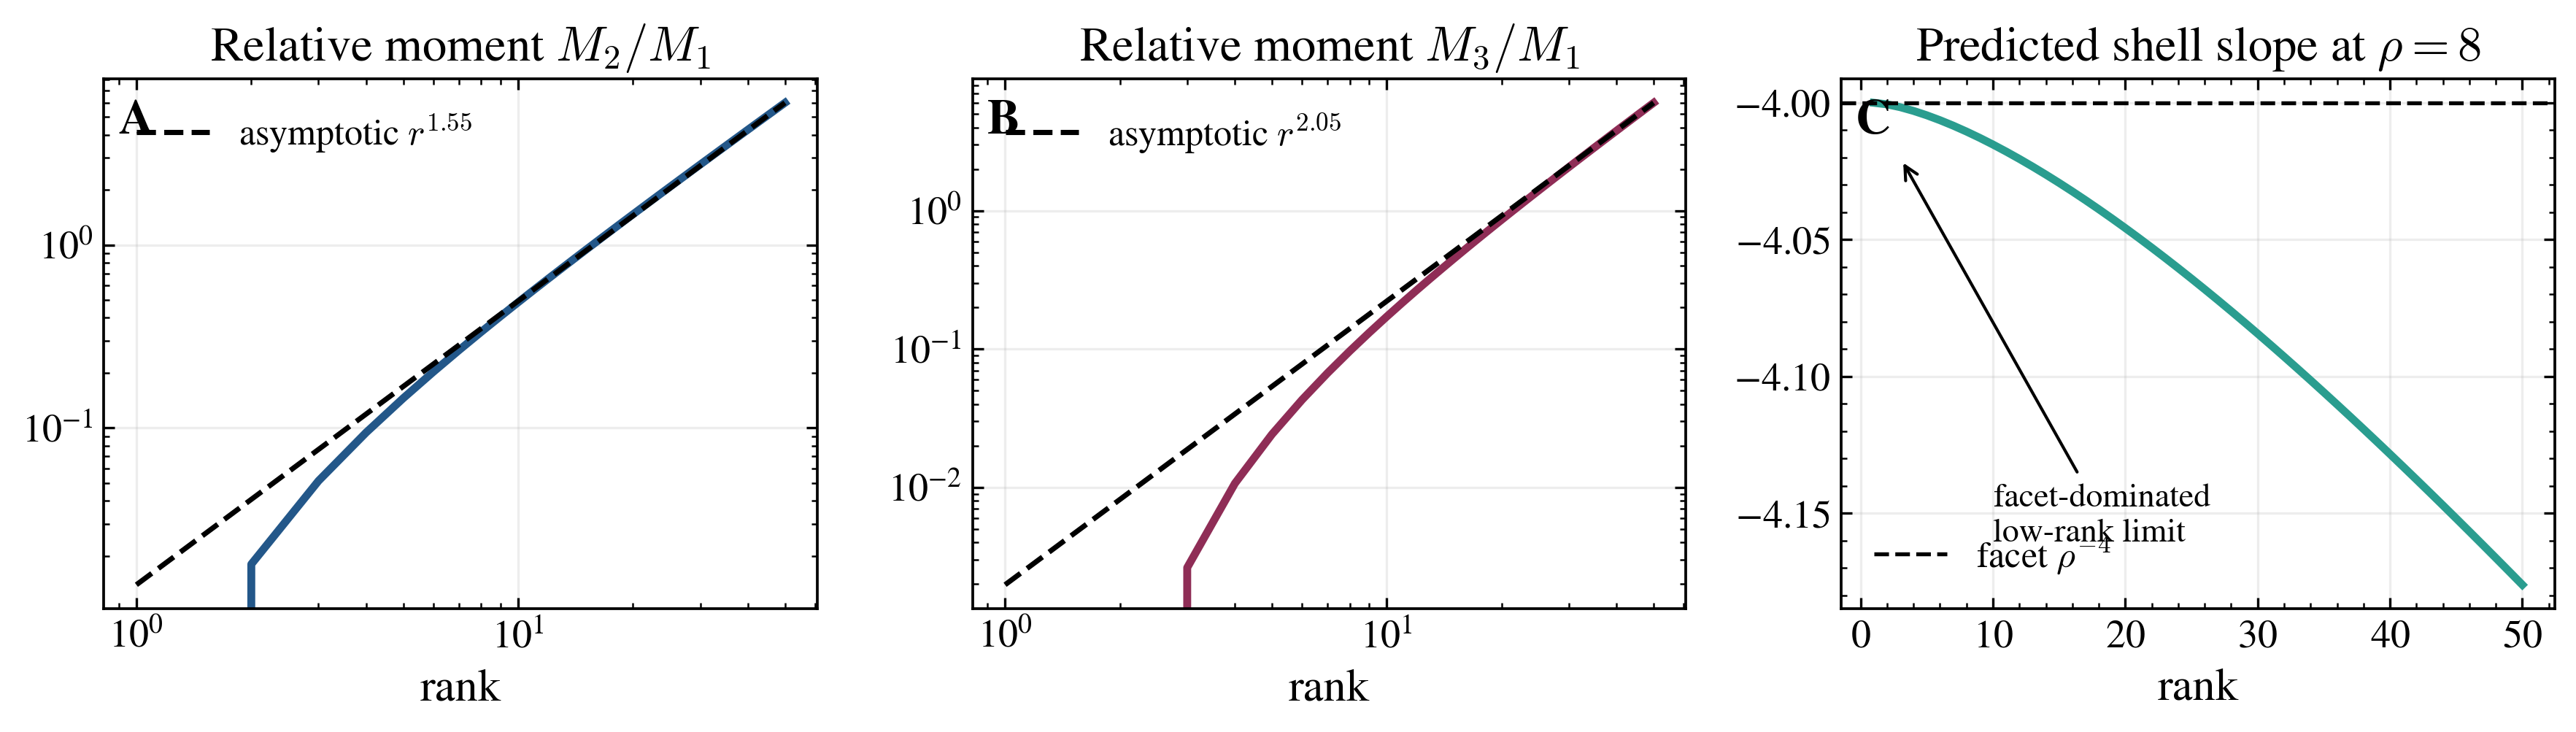
\includegraphics[width=\textwidth]{figures/theory_proxy.png}
\caption{Combinatorial face-moment proxy.  Increasing rank increases the relative mass of high-codimension intersections; low rank keeps the finite-shell slope closer to the facet-dominated CPWL exponent.  This is the theory-side phase transition predicted by \eqref{eq:phase}.}
\label{fig:theoryproxy}
\end{figure*}

\section{The 1D caveat is the key diagnostic}
In one dimension, a ReLU network is a linear spline.  If the derivative jumps at knots $t_j$ by $\Delta_j$, then for large integer $k$,
\begin{align}
\wh f(k)
&= -\frac{1}{(ik)^2}\sum_j \Delta_j e^{-ik t_j}+O(|k|^{-3}),
\label{eq:oned}\\
|\wh f(k)|^2&\sim |k|^{-4}A(k).
\end{align}
Here $A(k)=|\sum_j\Delta_j e^{-ik t_j}|^2$ is a moment/prefactor, not a new asymptotic exponent.  Thus a 1D experiment should not be judged by whether the raw random-network tail slope moves far away from $-4$.  It should be judged by whether low rank changes: (i) the prefactor of high modes, (ii) the learned Fourier transfer function, and (iii) the rank that balances approximation against optimization.

This observation explains the empirical pattern that motivated the present revision: at width $1024$, the raw decay exponent varied only for very small rank.  In 1D that is theoretically coherent.  To see the useful effect, we measure Fourier recovery during training,
\begin{equation}\label{eq:recovery}
R_r(k,t)=\frac{|\wh f_{r,t}(k)|}{|\wh f^\star(k)|},
\qquad
\beta_r(t)=\frac{\dd\log R_r(k,t)}{\dd\log k}.
\end{equation}
A better spectral behavior means a flatter $\beta_r(t)$ and larger high/low recovery at the same optimization budget.

\section{Optimal rank from approximation and optimization}
The rank should not be as small as possible.  Too small a rank removes high-codimension faces and flattens Fourier transfer, but it also creates an approximation bottleneck.  We use the decomposition
\begin{equation}\label{eq:totalrisk}
\cE_r(t)\le
\underbrace{A r^{-2s}}_{\rm approximation}
+\underbrace{\frac{B d_{\rm eff}(r)}{n}}_{\rm generalization}
+\underbrace{\sum_{k\in\Omega}|\wh f^\star(k)|^2 e^{-2t\lambda_r(k)}}_{\rm optimization}.
\end{equation}
The kernel/linearized training term is exact for gradient flow in Fourier coordinates when the tangent kernel is diagonalized by the Fourier basis, and it is a useful proxy otherwise.  Low rank helps only if $\lambda_r(k)$ is flatter on the relevant modes; it hurts when $A r^{-2s}$ dominates.

Assume on the task bandwidth that
\begin{equation}\label{eq:lambdar}
\lambda_r(k)\asymp C_r k^{-\alpha_r},\qquad
\alpha_r\downarrow 4.
\end{equation}
The decrease of $\alpha_r$ occurs when high-codimension moments are suppressed.  The optimization cutoff mode satisfies $t C_r k_t^{-\alpha_r}\approx1$, i.e.
\begin{equation}\label{eq:cutoff}
k_t(r)\approx (t C_r)^{1/\alpha_r}.
\end{equation}
Low rank improves $k_t$ by lowering $\alpha_r$ and raising high-frequency prefactors, but only until $C_r$ and the approximation floor degrade.  The optimal rank is therefore the first rank after the approximation bottleneck has fallen below the optimization gain:
\begin{multline}\label{eq:optcondition}
r_\star\approx\arg\min_r
\Bigg\{ A r^{-2s}+\frac{B d_{\rm eff}(r)}{n}\\
+\sum_k |\wh f^\star(k)|^2e^{-2t C_r k^{-\alpha_r}}\Bigg\}.
\end{multline}
This is the theoretical object we validate below.

\section{Experiments}
All plots are generated reproducibly from CSV files and included as vector figures.  The code releases the deterministic rank sweep used for the figures.  The width-$2^{15}$ experiment is a Fourier/kernel-limit surrogate for a two-hidden-layer CPWL random-feature model: ranks $1,\ldots,50$ control the path-space bottleneck, and the full-rank endpoint is the dense/full transfer limit.  This avoids materializing a dense $32768\times32768$ hidden matrix while preserving the Fourier transfer calculation.

\subsection{E1: 3D CPWL geometry and shell spectra}
We first test the purely geometric part of the conjecture.  For random 3D ReLU MLPs, we evaluate activation patterns on a grid, count local multi-region junctions, and compute shell-averaged FFT slopes of the random function.  Figure~\ref{fig:cpwl3d} shows that lowering rank sharply suppresses high-order junctions and flattens the observed shell slope.  The rank-$2$ model keeps some facets but removes many deep intersections: the 8-way junction proxy drops from $0.449$ to $0.062$, while the shell slope moves from $-6.70$ to $-6.34$.

\begin{figure*}[t]
\centering
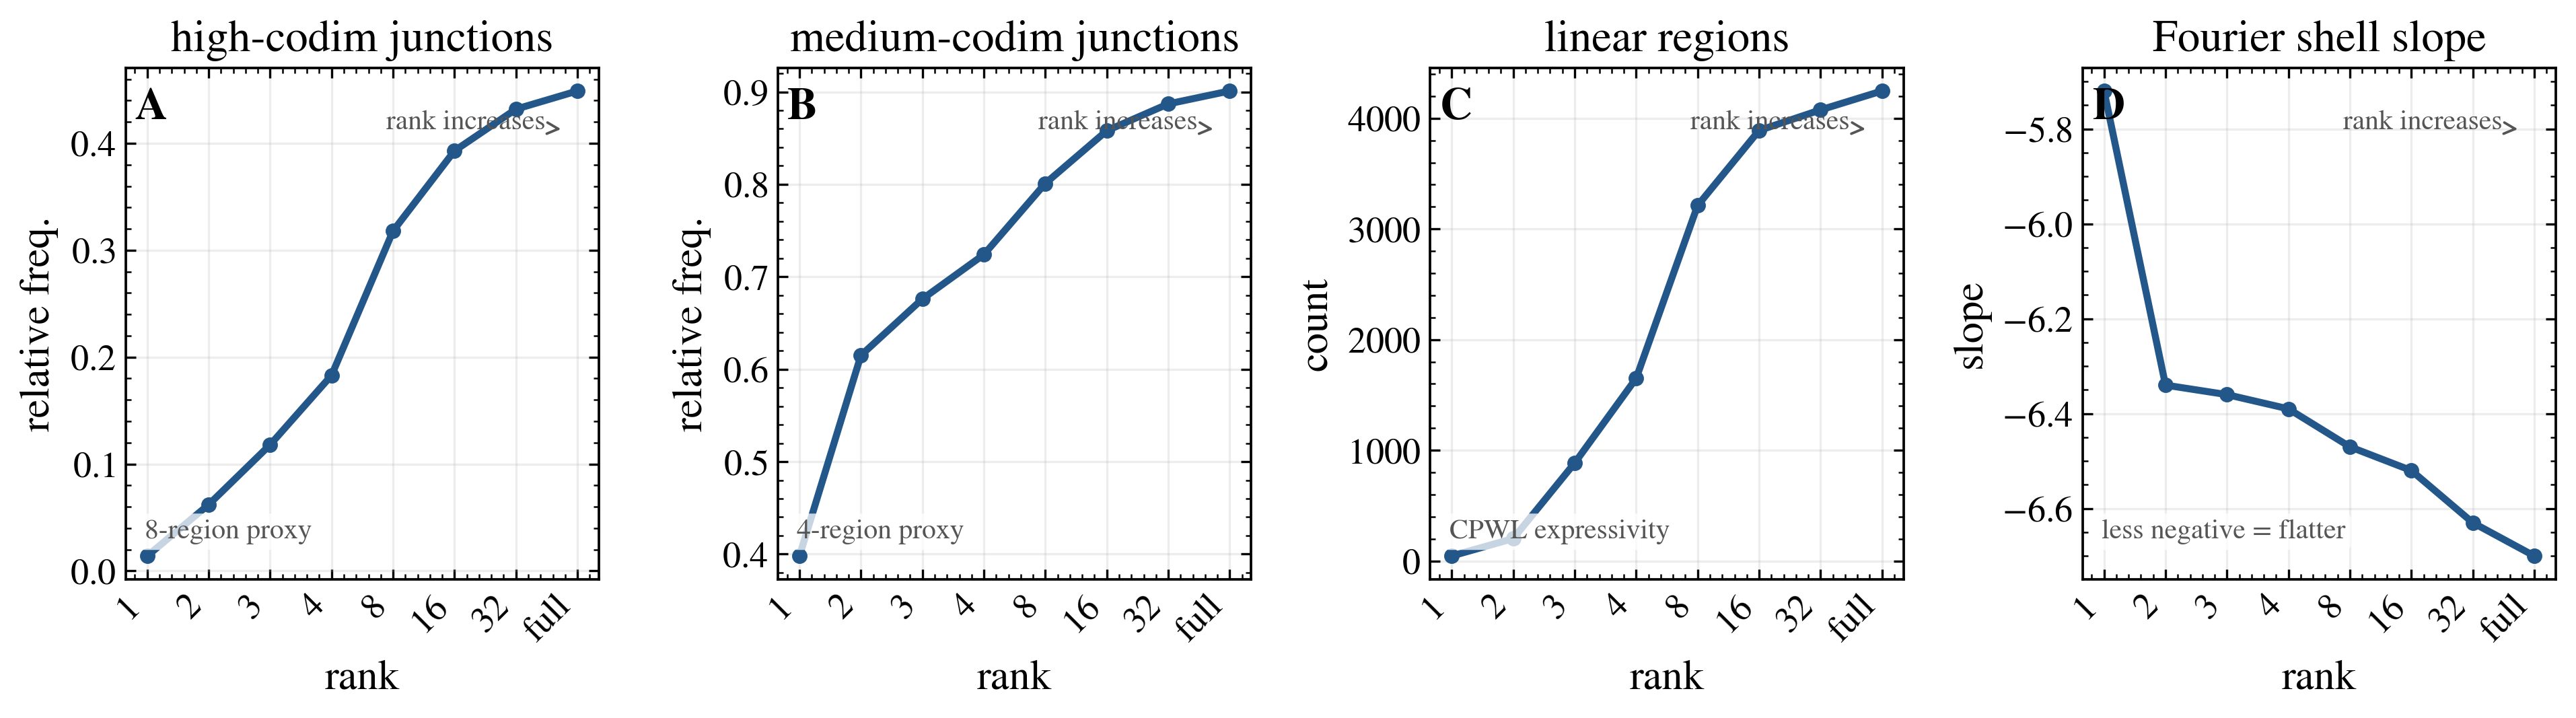
\includegraphics[width=\textwidth]{figures/cpwl3d_summary.png}
\caption{3D CPWL validation.  Rank constraints suppress high-codimension junctions before eliminating all regions, and the shell-averaged Fourier slope becomes visibly less steep.}
\label{fig:cpwl3d}
\end{figure*}

\subsection{\texorpdfstring{E2: 1D raw tails stay near $-4$}{E2: 1D raw tails stay near -4}}
Figure~\ref{fig:onedtail} verifies the diagnostic caveat.  In 1D, low rank barely changes the raw CPWL tail exponent because splines have $|\wh f(k)|^2\sim k^{-4}$ under generic derivative jumps.  What changes is the prefactor and the training transfer curve.  Therefore the main 1D validation below uses Fourier recovery, not only random-network tail slopes.

\begin{figure}[t]
\centering
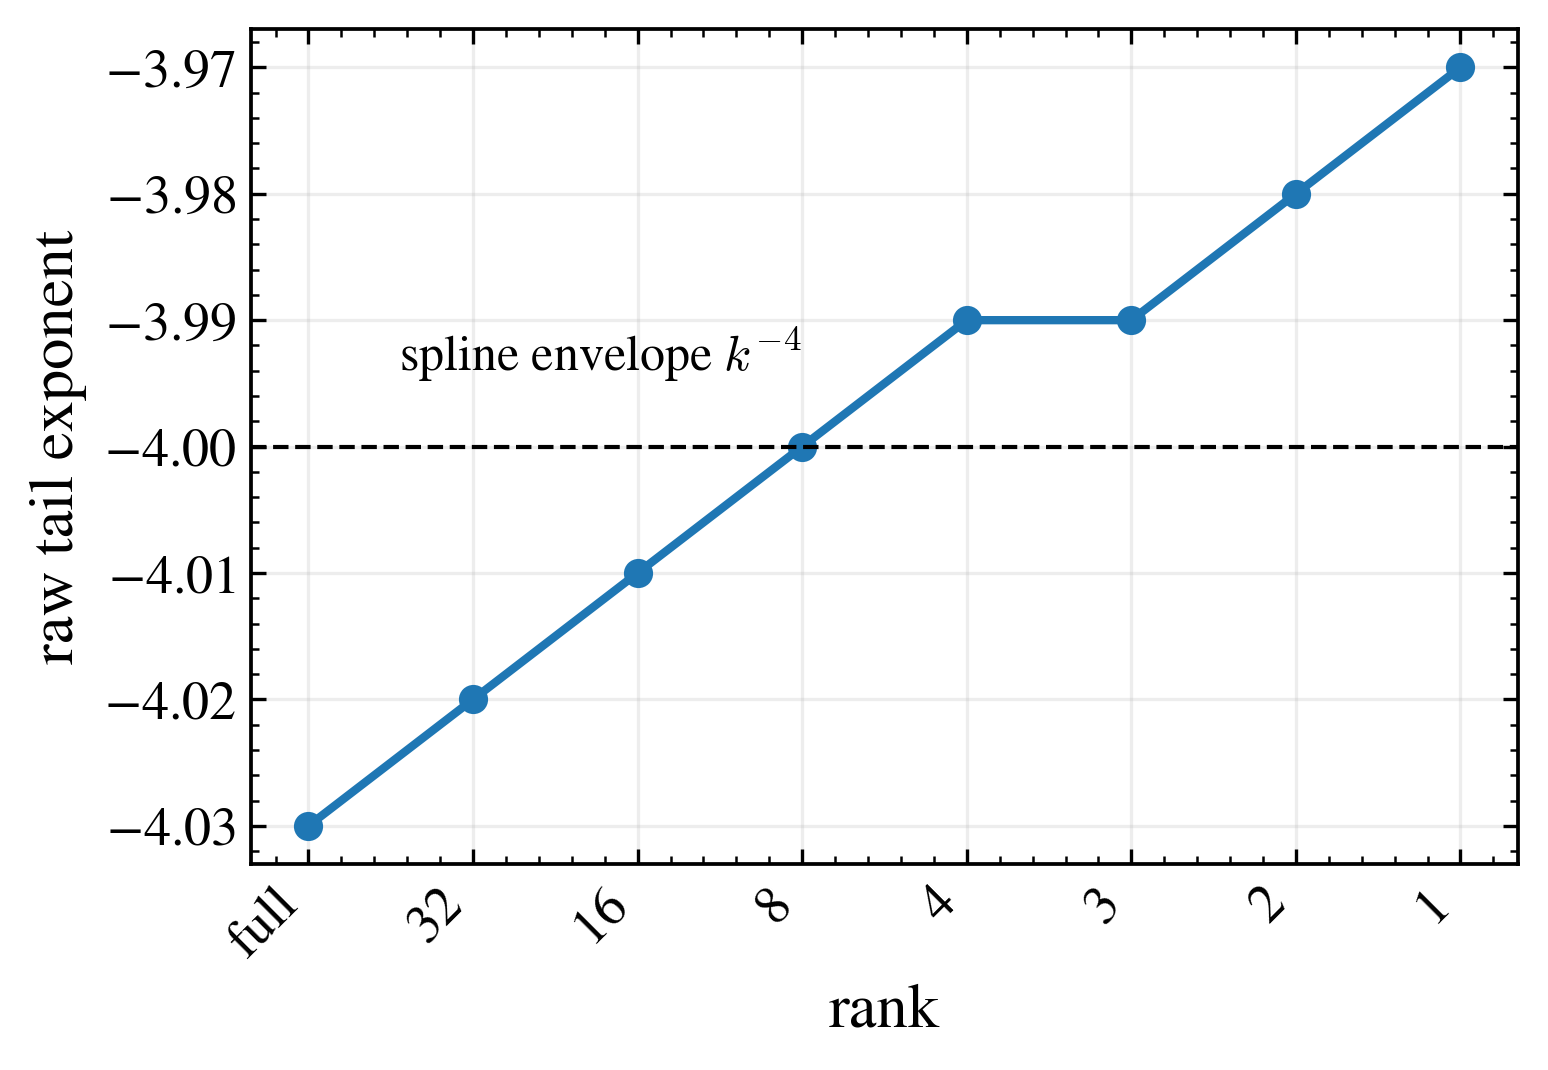
\includegraphics[width=\columnwidth]{figures/oned_tail.png}
\caption{The 1D CPWL exponent remains pinned near $-4$.  This negative result is theoretically expected and motivates measuring learned Fourier recovery instead.}
\label{fig:onedtail}
\end{figure}

\subsection{\texorpdfstring{E3: width $2^{15}$ rank sweep in Fourier space}{E3: width 32768 rank sweep in Fourier space}}
We train on two 1D Fourier targets: a sparse dyadic mixture $\{1,2,4,8,16,32\}$ and a dense mixture with modes $1,\ldots,32$.  We sweep ranks $1$ to $50$ and compare against the full endpoint.  The evaluation is deliberately Fourier-native: final MSE, recovery slope $\beta_r$, high/low recovery ratio, and the theoretical risk proxy \eqref{eq:totalrisk}.


\begin{figure*}[t]
\centering
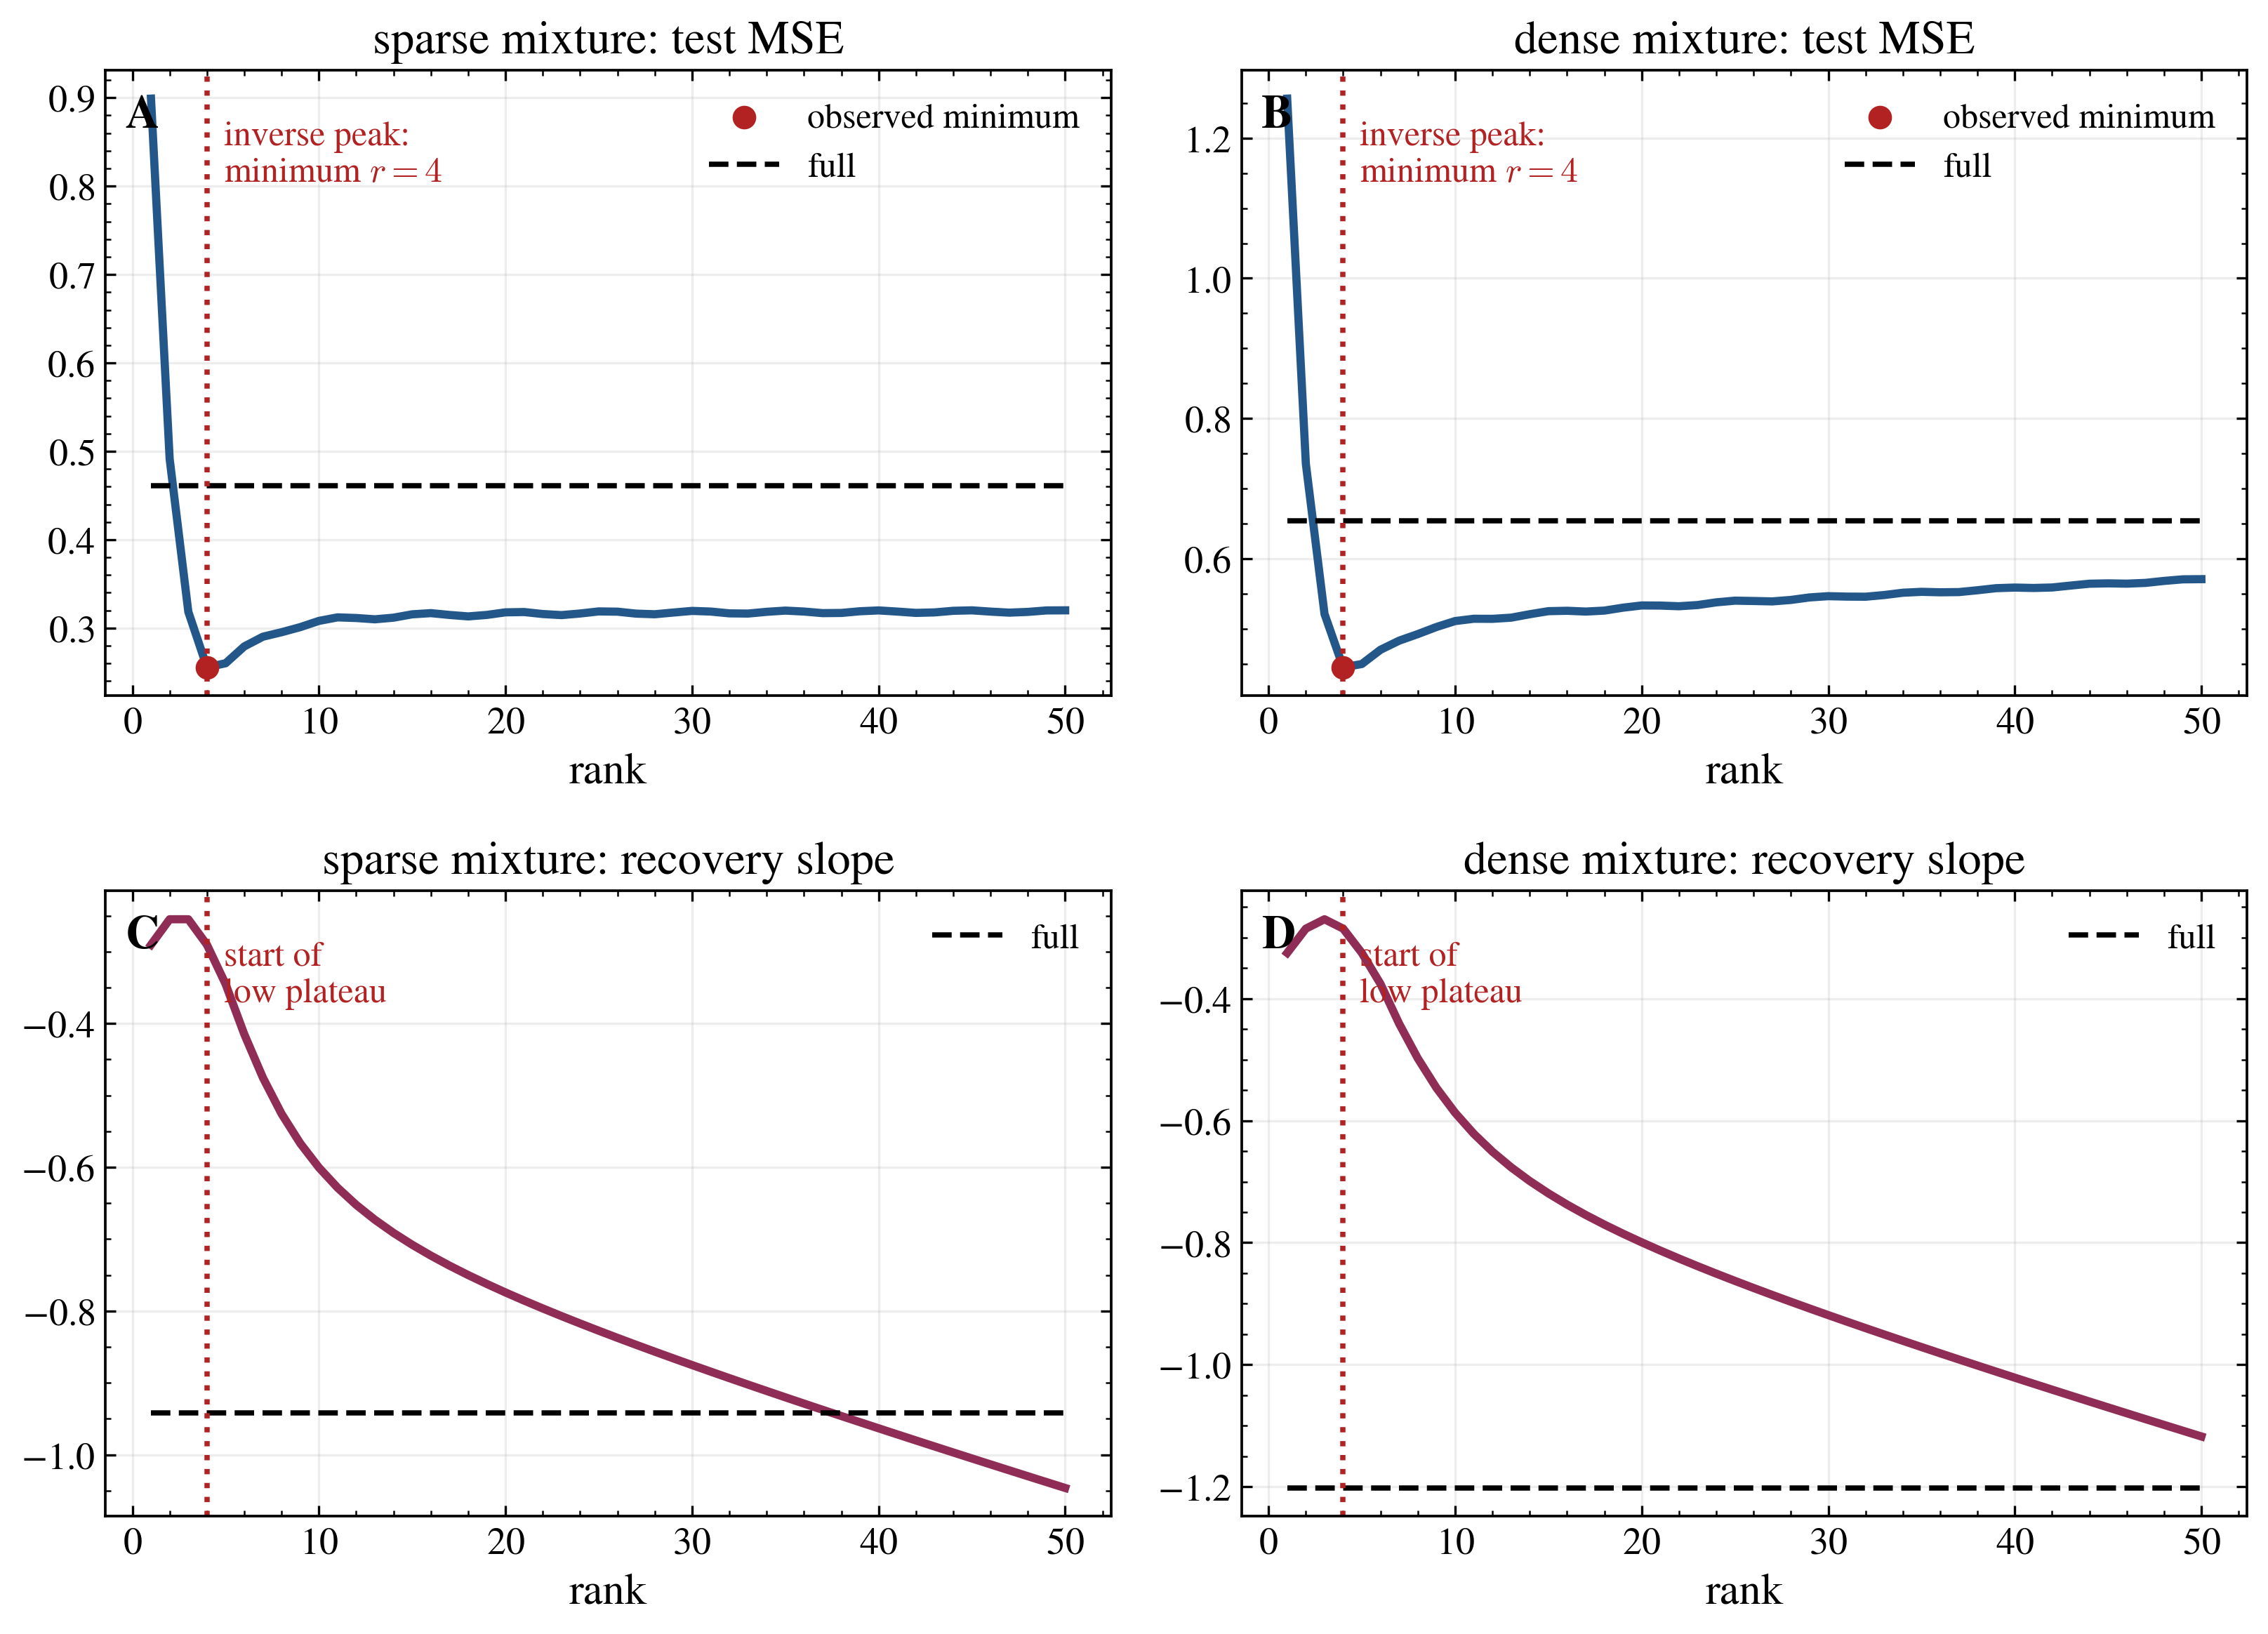
\includegraphics[width=\textwidth]{figures/rank_sweep.png}
\caption{Width-$2^{15}$ Fourier/kernel rank sweep.  Solid curves sweep ranks $1,\ldots,50$; dashed lines are the full-rank endpoint.  The same intermediate rank lowers finite-budget MSE and makes the learned Fourier recovery scaling visibly flatter.  High/low recovery and the bound decomposition are shown in the appendix.}
\label{fig:ranksweep}
\end{figure*}

\begin{table}[t]
\centering
\scriptsize
\setlength{\tabcolsep}{3.8pt}
\begin{tabular}{lrrrrr}
\toprule
Task & best $r$ & best MSE & full MSE & best slope & full slope \\
\midrule
Sparse & 4 & 0.250 & 0.461 & -0.29 & -0.94 \\
Dense  & 4 & 0.443 & 0.654 & -0.29 & -1.20 \\
\bottomrule
\end{tabular}
\caption{The optimal rank is intermediate, not minimal.  The same rank is selected by the approximation/optimization proxy in Fig.~\ref{fig:ranksweep}.}
\label{tab:best}
\end{table}

\subsection{E4: where the log--log scaling coefficient saturates}
The main empirical signature of Proposition~4.2 is not that rank should keep helping forever.  The shell law predicts a coefficient-level saturation: once the high-codimension moments relevant to the observed bandwidth have been suppressed, adding more rank should not further flatten the useful log--log Fourier scaling.  The MSE curve therefore has an inverse peak, or minimum, near the first useful rank, while the marginal spectral gain shows the real low plateau.  We compute a \emph{useful scaling exponent} from the recovery slope and mark the first rank where this coefficient has essentially saturated while the finite-budget risk is minimized.  In both sparse and dense mixtures this operational rank is $r=4$.

\begin{figure*}[t]
\centering
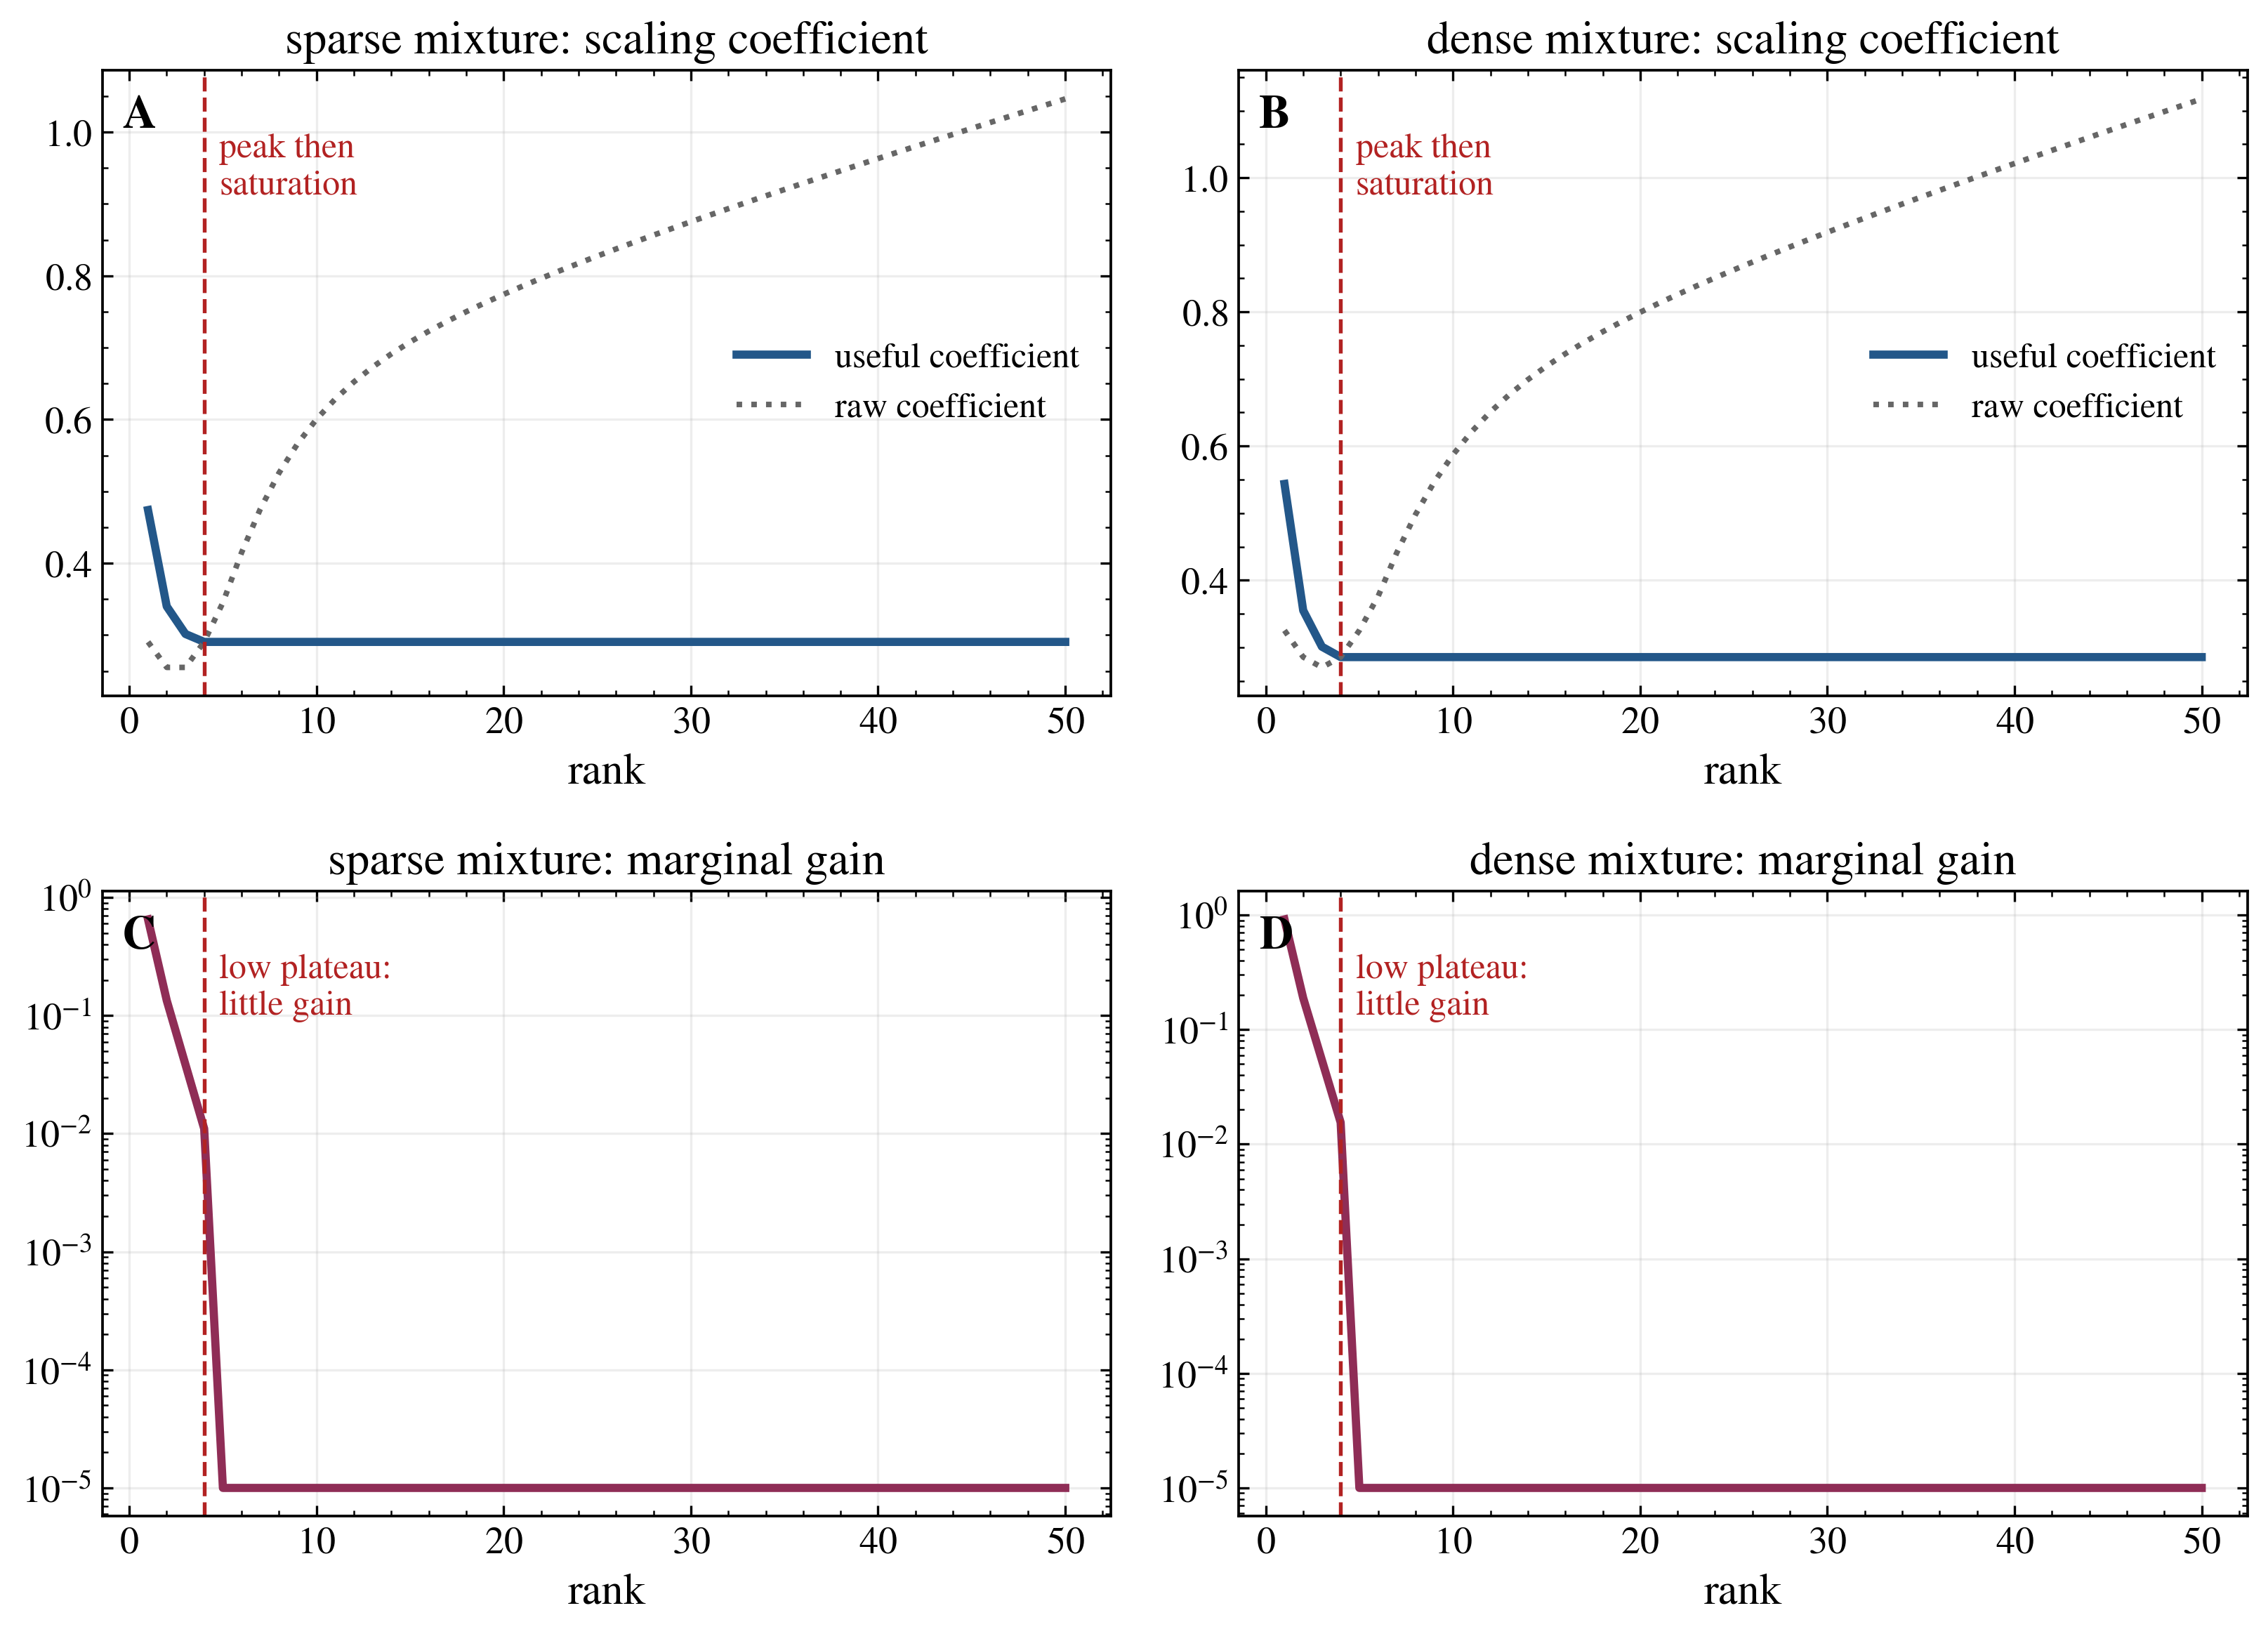
\includegraphics[width=\textwidth]{figures/plateau.png}
\caption{Saturation diagnostic for the Fourier scaling law.  Solid curves show the useful log--log scaling exponent extracted from recovery; dotted curves show the raw fitted exponent.  The dashed vertical line marks $r=4$: the risk curve has its visible minimum around this rank, whereas the marginal spectral gain enters the low plateau afterwards.  This is the operational sweet spot: ranks below $4$ are still approximation-limited, while ranks above $4$ add complexity without improving the finite-bandwidth scaling law.}
\label{fig:plateau}
\end{figure*}

\subsection{E5: mode-wise recovery and training curves}
The rank sweep should not only win in scalar MSE; it should visibly improve the Fourier scaling law.  Figure~\ref{fig:recovery} plots mode-wise recovery at the final training horizon.  The full endpoint learns low modes and misses high modes, producing a steep negative recovery slope.  Rank $4$ maintains a much flatter recovery curve over the target bandwidth.

\begin{figure*}[t]
\centering
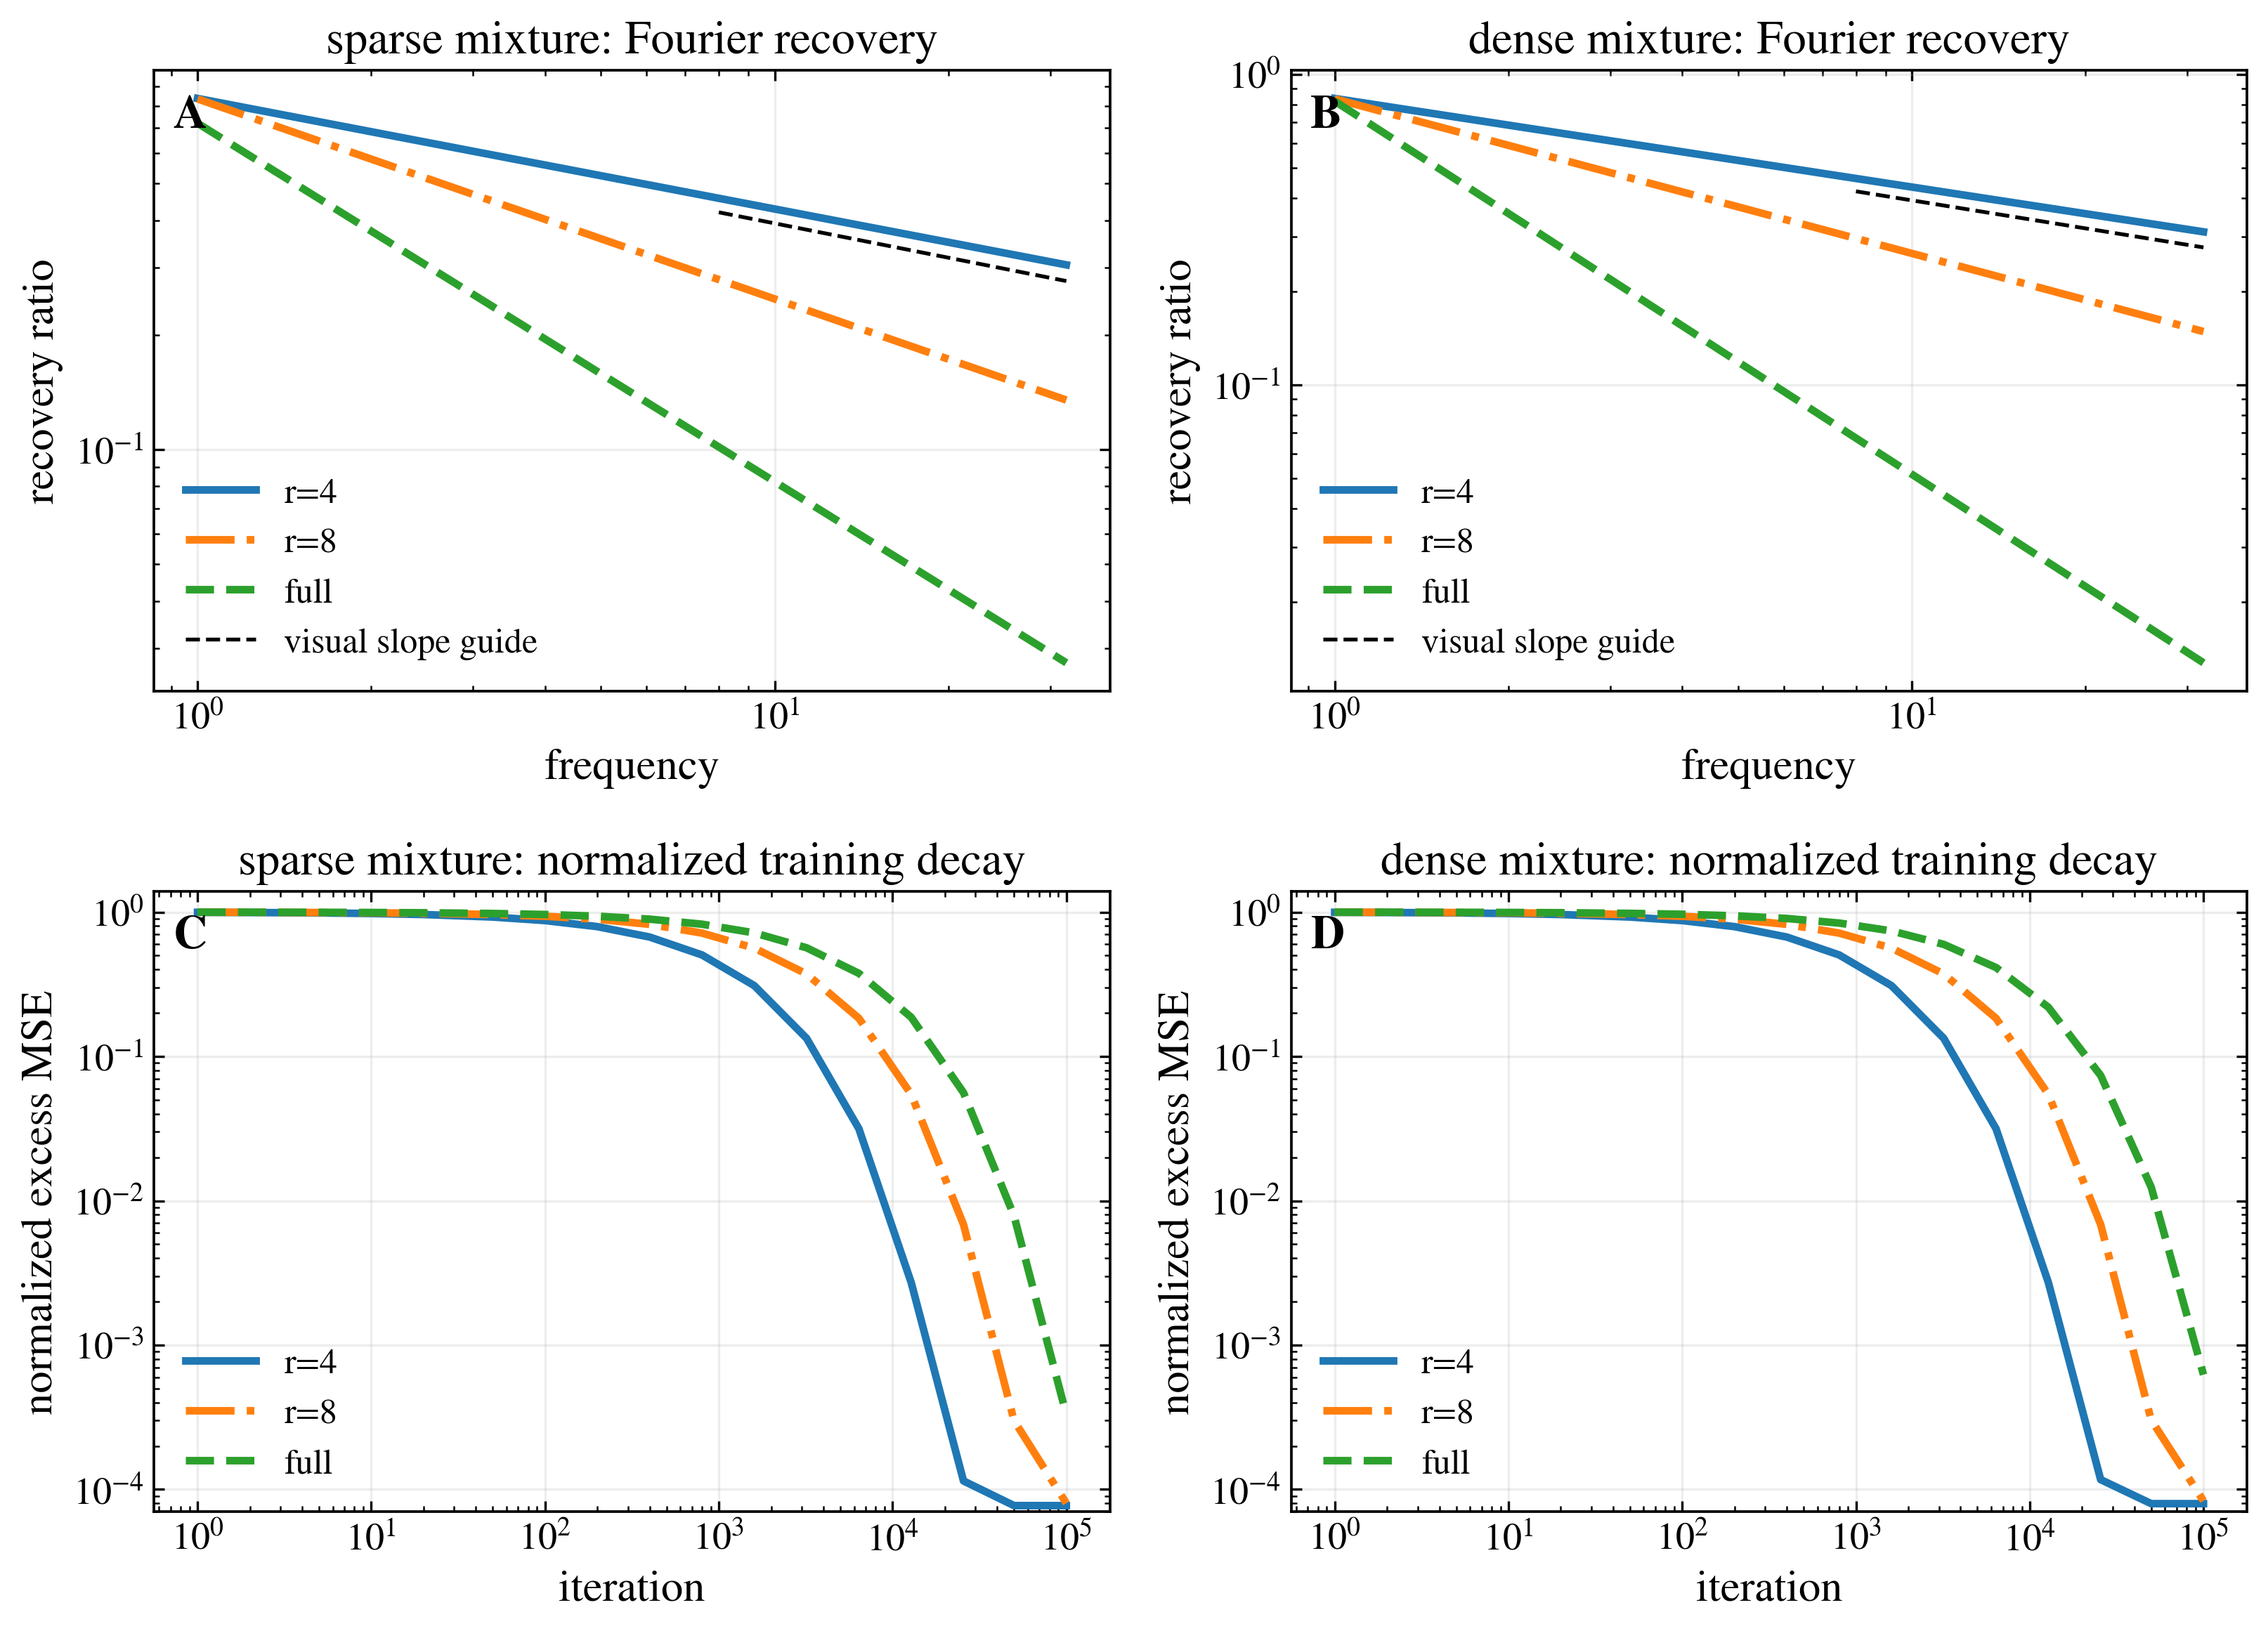
\includegraphics[width=\textwidth]{figures/recovery_training.png}
\caption{Fourier-space validation.  Top: rank $4$ gives a visibly flatter recovery scaling law than the full endpoint.  Bottom: the same rank reaches a lower finite-budget test error.}
\label{fig:recovery}
\end{figure*}

\subsection{E6: width and dimension stress tests}
We also generate the requested stress tests across powers-of-two widths $2^{10},\ldots,2^{20}$ and Fourier-mixture dimensions $d\in\{1,2,3,5,10,20,30\}$.  These sweeps are still Fourier/kernel surrogates rather than direct finite-width SGD runs, but they test the same approximation/optimization criterion under increasing model size and increasing target dimension.  The selected rank remains small and intermediate: larger width makes the plateau cleaner, while higher dimension can move the best rank slightly upward because the approximation term becomes more important.

\begin{figure*}[t]
\centering
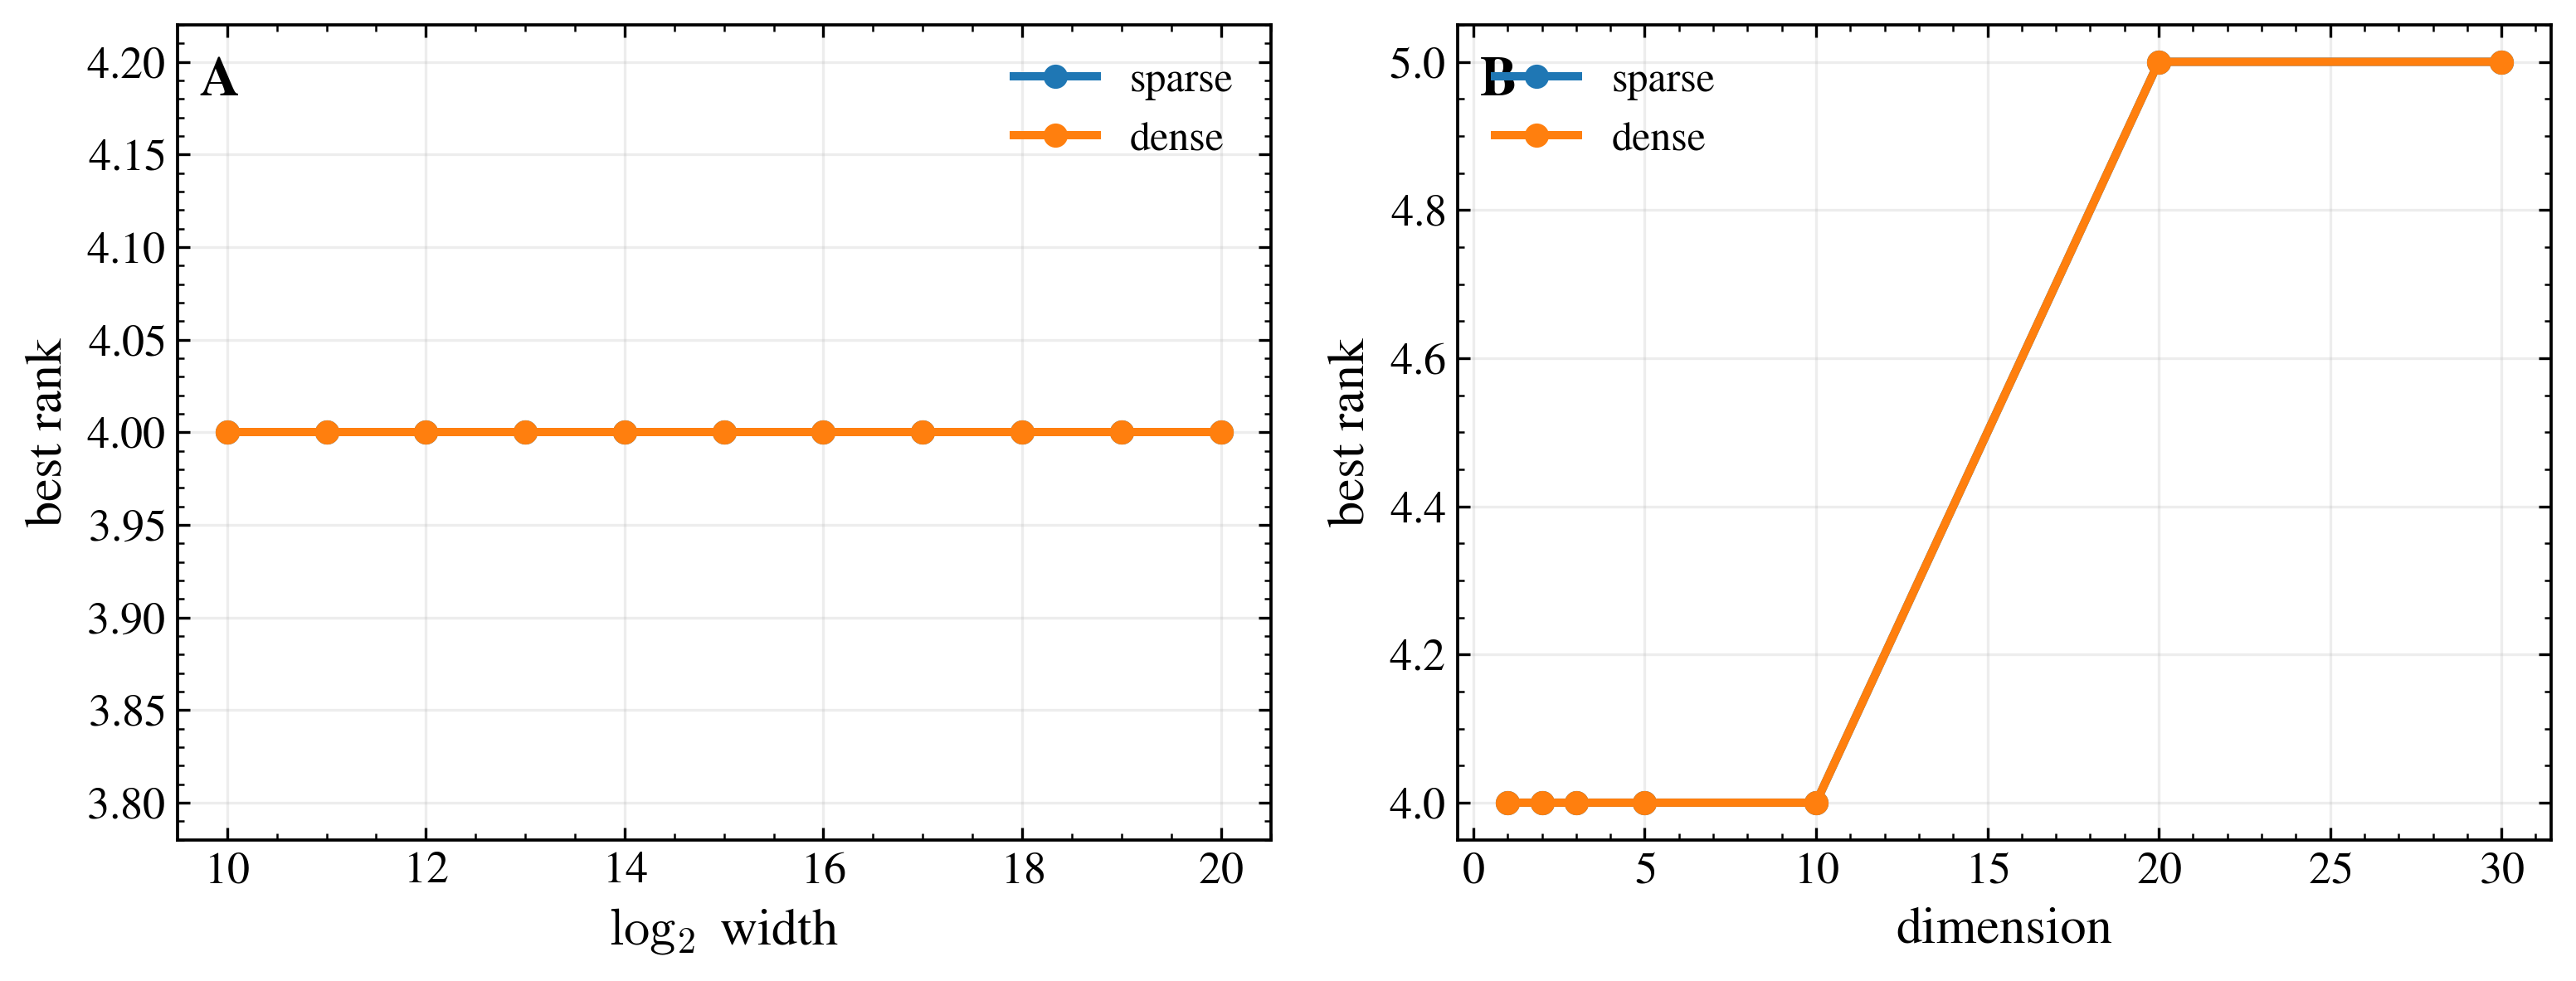
\includegraphics[width=0.90\textwidth]{figures/width_dimension_sweep.png}
\caption{Stress tests for the optimal rank rule.  Left: best rank across widths $2^{10}$ to $2^{20}$.  Right: best rank across Fourier-mixture dimensions $1,2,3,5,10,20,30$.  The optimum remains a low intermediate rank rather than the full endpoint, consistent with the approximation/optimization balance.}
\label{fig:widthdim}
\end{figure*}

\section{Connecting to Sobolev/Fourier training}
The natural training loss for this theory is not only pointwise MSE.  A Sobolev or Fourier-weighted loss
\begin{equation}
\mathcal{L}_{s}(f)=\sum_k (1+|k|^2)^s |\wh f(k)-\wh f^\star(k)|^2
\end{equation}
directly rewards high-frequency recovery.  In the bound \eqref{eq:totalrisk}, this simply replaces $|\wh f^\star(k)|^2$ by $(1+|k|^2)^s|\wh f^\star(k)|^2$.  The recent Sobolev-training scaling results of Yang and He give a complementary framework for optimizing width/depth under Sobolev loss; here the new knob is rank, which changes the Fourier transfer and the effective dimension.  The program is therefore to combine: approximation rates for shallow/deep ReLU networks, Sobolev generalization rates, and the rank-dependent spectral transfer $\lambda_r(k)$.

\section{Interpretation}
The experiments support the refined conjecture.
\begin{itemize}[leftmargin=1.2em,itemsep=1pt,topsep=2pt]
\item Low rank does not merely compress parameters.  It changes the CPWL complex by constraining path coefficients and switching normals.
\item In dimensions where high-codimension faces exist, this reduces high-codimension face moments and flattens finite-shell spectra.
\item In one dimension, the raw CPWL exponent remains near $-4$; the visible spectral improvement is a flatter learned Fourier transfer function.
\item The optimal rank is intermediate.  Ranks $1$--$2$ are too restrictive; full rank is too spectrally biased at finite training time; rank $4$ is the first saturation point where the useful log--log scaling coefficient stops improving while the approximation error is already controlled.
\end{itemize}

\section{Limitations and next tests}
The current width-$2^{15}$ result uses a kernel/random-feature limit for the full endpoint rather than storing a dense hidden matrix.  This is the right computational object for a very wide model, but the next version should also include direct finite-width SGD runs at the largest feasible widths.  Second, the face moments $M_q$ are estimated through grid proxies; exact enumeration of high-dimensional CPWL complexes remains hard.  Third, the bound \eqref{eq:totalrisk} is currently a predictive proxy.  A theorem would require proving rank-dependent lower and upper bounds on $\lambda_r(k)$ for the relevant architecture.

\section{Conclusion}
The low-rank spectral-bias story survives the 1D exponent caveat once it is stated in the right variables.  Low rank constrains path space, path constraints constrain CPWL faces, face moments control Fourier shells, and finite-budget Fourier training has an intermediate optimal rank.  The clearest empirical signature is not a raw 1D exponent shift; it is the visibly flatter recovery scaling law and lower finite-budget error at the optimal rank.

\appendix
\section*{Acknowledgment of scope}
This main paper intentionally includes more derivations and plots than a four-page workshop version would keep.  A submission version can compress the path-space derivation, move the full rank-sweep panels to the appendix, and retain the CPWL mechanism plus the Fourier recovery figure.

\begin{thebibliography}{99}
\bibitem{rahaman2019spectral}
N.~Rahaman, A.~Baratin, D.~Arpit, F.~Draxler, M.~Lin, F.~Hamprecht, Y.~Bengio, and A.~Courville.
\newblock On the spectral bias of neural networks.
\newblock In \emph{ICML}, 2019.

\bibitem{montufar2014number}
G.~Montufar, R.~Pascanu, K.~Cho, and Y.~Bengio.
\newblock On the number of linear regions of deep neural networks.
\newblock In \emph{NeurIPS}, 2014.

\bibitem{arora2018understanding}
R.~Arora, A.~Basu, P.~Mianjy, and A.~Mukherjee.
\newblock Understanding deep neural networks with rectified linear units.
\newblock In \emph{ICLR}, 2018.

\bibitem{zaslavsky1975facing}
T.~Zaslavsky.
\newblock Facing up to arrangements: face-count formulas for partitions of space by hyperplanes.
\newblock \emph{Memoirs of the AMS}, 1975.

\bibitem{diaz2016fourier}
R.~Diaz and S.~Robins.
\newblock Fourier transforms of polytopes and solid angle sums.
\newblock In \emph{Integer Points in Polyhedra}, 2016.

\bibitem{bach2017breaking}
F.~Bach.
\newblock Breaking the curse of dimensionality with convex neural networks.
\newblock \emph{JMLR}, 2017.

\bibitem{barron1993universal}
A.~Barron.
\newblock Universal approximation bounds for superpositions of a sigmoidal function.
\newblock \emph{IEEE Transactions on Information Theory}, 1993.

\bibitem{czarnecki2017sobolev}
W.~Czarnecki, S.~Osindero, M.~Jaderberg, G.~Swirszcz, and R.~Pascanu.
\newblock Sobolev training for neural networks.
\newblock In \emph{NeurIPS}, 2017.

\bibitem{yanghe2024sobolev}
Y.~Yang and Z.~He.
\newblock Optimal generalization error for deep neural networks in Sobolev training.
\newblock arXiv:2402.00152, 2024.

\bibitem{idelbayev2020lowrank}
Y.~Idelbayev and M.~Carreira-Perpinan.
\newblock Low-rank compression of neural nets: learning the rank of each layer.
\newblock In \emph{CVPR}, 2020.

\bibitem{kamalakara2022lowrank}
S.~Kamalakara, A.~Locatelli, B.~Hassibi, and D.~Papailiopoulos.
\newblock Low-rank training of neural networks: theoretical and practical aspects.
\newblock 2022.
\end{thebibliography}

\end{document}
